\iffalse

INSTRUCTIONS: (if this is not lecture1.tex, use the right file name)

  Clip out the ********* INSERT HERE ********* bits below and insert
appropriate TeX code.  Once you are done with your file, run

  ``latex lecture1.tex''

from a UNIX prompt.  If your LaTeX code is clean, the latex will exit
back to a prompt.  Once this is done, run

  ``dvips lecture1.dvi''

which should print your file to the nearest printer.  There will be
residual files called lecture1.log, lecture1.aux, and lecture1.dvi.
All these can be deleted, but do not delete lecture1.tex.
\fi
%
\documentclass[11pt]{article}
\usepackage{amsfonts}
\usepackage{amsmath}
\usepackage{latexsym}
\usepackage{hyperref}
\usepackage{tikz}
\usepackage{listings}
%\usepackage{tikz-qtree}
\usetikzlibrary{automata,arrows}


\hypersetup{
    colorlinks=true,
    linkcolor=blue,
    filecolor=magenta,      
    urlcolor=cyan,
}
 
\urlstyle{same}

\setlength{\oddsidemargin}{.25in}
\setlength{\evensidemargin}{.25in}
\setlength{\textwidth}{6in}
\setlength{\topmargin}{-0.4in}
\setlength{\textheight}{8.5in}

\newcommand{\handout}[5]{
   %\renewcommand{\thepage}{#1-\arabic{page}}
   \noindent
   \begin{center}
   \framebox{
      \vbox{
    \hbox to 5.78in { {\bf Data Structures and Algorithms} \hfill #2 }
       \vspace{4mm}
       \hbox to 5.78in { {\Large \hfill #5  \hfill} }
       \vspace{2mm}
       \hbox to 5.78in { {\it #3 \hfill #4} }
      }
   }
   \end{center}
   \vspace*{4mm}
}

\newcommand{\lecture}[3]{\handout{L#1}{#2}{}{}{#1}}

\def\squarebox#1{\hbox to #1{\hfill\vbox to #1{\vfill}}}
\def\qed{\hspace*{\fill}
        \vbox{\hrule\hbox{\vrule\squarebox{.667em}\vrule}\hrule}}
\newenvironment{solution}{\begin{trivlist}\item[]{\bf Solution:}}
                      {\qed \end{trivlist}}
\newenvironment{solsketch}{\begin{trivlist}\item[]{\bf Solution Sketch:}}
                      {\qed \end{trivlist}}
\newenvironment{proof}{\begin{trivlist}\item[]{\bf Proof:}}
                      {\qed \end{trivlist}}

\newtheorem{theorem}{Theorem}
\newtheorem{corollary}[theorem]{Corollary}
\newtheorem{lemma}[theorem]{Lemma}
\newtheorem{observation}[theorem]{Observation}
\newtheorem{remark}[theorem]{Remark}
\newtheorem{proposition}[theorem]{Proposition}
\newtheorem{definition}[theorem]{Definition}
\newtheorem{Assertion}[theorem]{Assertion}
\newtheorem{fact}[theorem]{Fact}
\newtheorem{hypothesis}[theorem]{Hypothesis}
%\newtheorem{observation}[theorem]{Observation}
%\newtheorem{proposition}[theorem]{Proposition}
\newtheorem{claim}[theorem]{Claim}
\newtheorem{assumption}[theorem]{Assumption}

%Put more macros here, as needed.
\newcommand{\al}{\alpha}
\newcommand{\Z}{\mathbb Z}
\newcommand{\jac}[2]{\left(\frac{#1}{#2}\right)}
\newcommand{\set}[1]{\{#1\}}

\def\ppt{{\sf PPT}}
\def\poly{{\sf poly}}
\def\negl{{\sf negl}}
\def\owf{{\sf OWF}}
\def\owp{{\sf OWP}}
\def\tdp{{\sf TDP}}
\def\prg{{\sf PRG}}
\def\prf{{\sf PRF}}

%end of macros
\begin{document}

\fbox{
\vbox{
    \begin{flushleft}
        Hudson Cho, Ryan Wilson, Jesse Washburn, Colin Shuster, Samhith Patibandla\\  % authors' names
        COSC 336 \\  %class
        04/20/2025\\  % date
    \end{flushleft}
\center{\Large{\textbf{Assignment 7}}}
} % end vbox
} % end fbox
\vline

\textbf{Instructions.}
\begin{enumerate}
\item Due date and time: As indicated on Blackboard. 
\item This is a team assignment. Work in teams of 3-4 students.  Submit on Blackboard one assignment per team, with the names of all students making the team. 
\item The exercises will not be graded, but you still need to present your best attempt to solve them. If you do not know how to solve an exercise, say it.  This will give me feedback about your understanding of the theoretical concepts.
\item Your programs must be written in Java.

\item Write your programs neatly - imagine yourself grading your program and see if it is easy to read and understand. 

Comment your programs reasonably: there is no need to comment lines like "i++" but do include brief comments describing the main purpose of a specific block of lines.
\item  You will submit on \textbf{Blackboard} 2 files.  

The \textbf{1-st file} is a pdf file (produced ideally with latex and Overleaf) and it will contain the following:
\begin{enumerate}
\item The solution to the Exercises (see the remark above).
\item   A short description of your algorithm for the Programming Task, where you explain the dynamic programing approach. Focus on how you have modified MERGE.
\item   A table with the results your program gives  for the data sets indicated for the programming task. 
\item   The java code (so that the grader can make observations) of the  program.
\end{enumerate}


The \textbf{2-nd file} is the .java file containing the java source code for Programming Task.

\end{enumerate}
\newpage

\if01
\textbf{Instructions.}
\begin{enumerate}
\item Due date is announced on Blackboard.
\item This is a team assignment. Work in teams as in the previous assignments.  Submit one assignment per team, with the names of all students making the team.
\item Your programs must be written in Java.
\item Write your programs neatly - imagine yourself grading your program and see if it is easy to read and understand. 
At the very beginning present your algorithm in plain English or in pseudo-code (or both).
Comment your programs reasonably: there is no need to comment lines like "i++" but do include brief comments describing the main purpose of a specific block of lines.
\item  You will submit on Blackboard 2 files. The first file should be a .pdf file  with the solution to the exercises  and with  descriptions in English or in pseudocode of the algorithms  for the  programming task  you are required to do and the results that you are required to report.
Make sure you label the results as indicated below.   Also include in this pdf file, the JAVA code of your program so that the grader can make comments on it.
% Also insert images/screenshots with the output you obtain for each testing data. 
The second file  will contain  the  Java sources of your two programs.





%Staple all pages together.  You should have the electronic copy  of your programs with you (for example on a memory stick) because you may be asked to make a demo.

For editing the above document with  Latex, see the template posted on the course website. 
 
           assignment-template.tex	and
           
          assignment-template.pdf


To append in the  latex file  a pdf file, place it  in the same folder and then include them  in the latex file with 
\begin{verbatim}
\includepdf[pages=-,pagecommand={},width=\textwidth]{file.pdf}

\end{verbatim}
To append in the  latex file a .jpg file (for a photo), use 
\begin{verbatim}
\includegraphics[width=\linewidth]{file.jpg}

\end{verbatim}



\end{enumerate}
\newpage
\fi
%%%%%%%%%%%%%%%%%%%%%%


%%%%%%%%%%%%%%

\textbf{Exercise 1.} Show similarly to Fig 8.3 on page 212 in the textbook, how \textsf{RadixSort} sorts the following arrays:

\begin{enumerate}

\item 34, 9134, 20134, 29134, 4, 134


\begin{center}
\begin{tabular}{|c c c c c c |} 
 \hline
 Input & Ones & Tens & Hundreds & Thousands & Ten-Thousand \\ 
 \hline\hline
 00034 & - & 00004 & - &   00004 &  00004 \\ 
\hline
 09134 & - & 00034 &  - & 00034 & 00034\\ 
 \hline
 20134 & - & 09134  & - & 20134 & 00134 \\ 
 \hline
 29134 & - & 20134  & - &  00134 & 09134  \\ 
 \hline
 00004 & - & 29134 &  - & 09134 &  20134  \\ 
  \hline
  00134 & - & 00134  &  - &  29134 &  29134\\ 
  \hline
\end{tabular}
\end{center}


\item 4, 34, 134, 9134, 20134, 29134


\begin{center}
    
\begin{tabular}{|c c c c c c |} 
 \hline
 Input & Ones & Tens & Hundreds & Thousands & Ten-Thousand \\ 
 \hline\hline
 00004 & - & - & - &    00004 &  00004  \\ 
\hline
 00034 & - & - &  - & 00034 & 00034 \\ 
 \hline
 00134  & - & -  & - &  00134  &  00134  \\ 
 \hline
 09134 & - & -  & - &  20134 & 09134 \\ 
 \hline
 20134 & - & - &  - & 09134 &  20134  \\ 
  \hline
  29134 & - & -  &  - &  29134 &  29134 \\ 
  \hline
\end{tabular}
\end{center}


\item 29134, 20134, 9134, 134, 34, 4

\begin{center}
    
\begin{tabular}{|c c c c c c |} 
 \hline
 Input & Ones & Tens & Hundreds & Thousands & Ten-Thousand \\ 
 \hline\hline
 29134 & - & 00004 & 00004 &    00004 &  00004  \\ 
\hline
 20134 & - &29134 &   00034 & 00034 & 00034 \\ 
 \hline
 09134  & - & 20134  &29134 &  20134  &  00134  \\ 
 \hline
 00134 & - & 09134   & 20134&  00134 & 09134 \\ 
 \hline
 00034 & - & 00134& 09134  & 29134 &  20134  \\ 
  \hline
  00004 & - &  00034  & 00134 &  09134 &  29134 \\ 
  \hline
\end{tabular}
\end{center}

\end{enumerate}

\textbf{Exercise 2.} Present an $O(n)$ algorithm that sorts $n$ positive integer numbers  $a_1, a_2, \ldots, a_n$ which are known to be bounded by $n^2-1$ (so $0 \leq a_i \leq n^2-1$, for every $i=1, \ldots, n$. Use the idea of Radix Sort  (discussed in class and presented in Section 8.3 in the textbook).

Note that in order to obtain $O(n)$ you have to do Radix Sort by writing the numbers in a suitable base.  Recall that the runtime of Radix Sort is $O(d (n+k))$, where $d$ is the number of digits, and $k$ is the base, so that the number of digits in the base is also $k$. The idea is to represent each number in a base $k$ chosen so that  each number in $\{0,1, \ldots, n^2-1\}$  requires only $2$ ``digits," so $d=2$.   Explain what is the base that you choose and  how the digits of each number are calculated, in other words how you convert from base 10 to the base.  Note that you cannot use the base 10 representation, because $n^2-1$ (which is the largest possible value) requires $\log_{10} (n^2-1)$ digits in base $10$, which is obviously not constant and therefore you would not obtain an $O(n)$-time algorithm.   By the same argument we see that no base $k$ that is constant works, therefore $k$ has to depend on $n$.   In your explanations you need to indicate the formula that gives $k$ as a function of $n$, and show that $d=2$ ``digits'' are enough to represent all the numbers in the range $\{0,1, \ldots, n^2-1\}$.

Illustrate your algorithm by showing on paper similar to Fig. 8.3, page 198 in the textbook (make sure you indicate clearly the columns)  how the algorithm sorts the following 2 sequences: 
\smallskip

(a) 45, 98, 3, 82, 132, 71, 72, 143, 91, 28, 7, 45.

In this example $n=12$, because there are $12$ positive numbers in the sequence bounded by $143 = 12^2 - 1$. 
\smallskip

(b) 45, 98, 3, 82, 132, 71, 72, 143, 91, 28, 7, 45, 151, 175, 145, 399, 21, 267, 346, 292.

In this 2-nd example $n=20$, because there are $20$ positive numbers in the sequence bounded by $399= 20^2 - 1$. 
\bigskip

Note: if you use a base $b$ bigger than 10, you do not need to invent symbols for the digits larger than 10; instead use as digits the numbers $0,1, \ldots, b-1$ represented in base 10. For instance if you use base, say 25, the digits will be: 0,1, \ldots, 9, 10, 11, \ldots, 23, 24. So  we view `10', `11', etc., as a single symbol. For instance in this representation the number 9 23 written in base 25 has 2 digits: 9 and 23. 

\newpage




\textbf{Programming Task.}

 This is related to Exercise 22.1-5, page 593 in the textbook.  

Part (a). Write a program  that computes the adjacency list of the directed  graph $G^2$ defined in the exercise (but I also define it just below; this is called the square of $G$), given the adjacency list of the directed graph $G$. 
The promised definition: The graph $G^2$ has the same nodes as $G$, and $(u,v)$ is an edge of $G^2$ if and only if there is path of length $1$ or $2$ from $u$ to $v$.

For example if $G$ is the graph on the left, then $G^2$  is the graph on the right. As you can see $G^2$ has the edges of $G$ and in our example there are the extra edges $(0,2)$ and $(1,3)$, because there is a path of length $2$ from $0$ to $2$ and a path of length $2$ from $1$ to $3$.

\begin{tikzpicture}[>=stealth',shorten >=1pt,auto,node distance=2.0cm,scale=0.2][h]
%\begin{tikzpicture}[shorten >=1pt,auto,node distance=2.8cm]][h]
  \node[state] (0) {$0$};
  \node[state] (1) [right of =0] {$1$};
  \node[state] (2) [below of=0] {$2$};
   \node[state] (3) [below of =1] {$3$};
  \

  
  
  \path[->]
    (0) edge  (1)    
    (1) edge  (2) 
    (2) edge (3)
  
    ;
   
\end{tikzpicture}
\quad \quad \quad\quad\begin{tikzpicture}[>=stealth',shorten >=1pt,auto,node distance=2.0cm,scale=0.2][h]
%\begin{tikzpicture}[shorten >=1pt,auto,node distance=2.8cm]][h]
  \node[state] (0) {$0$};
  \node[state] (1) [right of =0] {$1$};
  \node[state] (2) [below of=0] {$2$};
 \node[state] (3) [below of =1] {$3$};
  \

  
  
  \path[->]
    (0) edge  (1)    
    (1) edge  (2) 
    (0)   edge (2)
(2) edge (3)
(1) edge (3)
    ;
   
\end{tikzpicture}


For the adjacency list, you \textbf{must} use the Java class \textsf{Adj\_List\_Graph} given in the file \textsf{Adj\_List\_Graph.java} (see \textsf{Test\_Adj.java} for a very simple example of using this class).

You will read the input graph $G$ from a file which contains 2 lines. The first line contains the number $n$ of vertices of the graph. The second line contains a sequence of $n^2$  bits (values $0$ and $1$). The $n$ nodes are labeled $0,1, \ldots, n-1$. If the $i \times n + j$-th  bit in the sequence is $1$, then there is an edge from node $i$ to node $j$, and if the $i \times n + j$-th bit in the sequence is $0$,  then there is no edge from node $i$ to node $j$. In other words, if the $n^2$  bits are indexed with indices $0, 1, \ldots, n^2-1$,  from the bit with index $k$, you compute $i=k/n$ and $j = k \pmod{n}$ and if bit with index $k$ is 1, then there exists an edge $(i,j)$, and if it is $0$, then there is no edge $(i, j)$. For example, the graph $G$ above has $n=4$ and the edges are given by the following $n^2 = 16$ bits: 0 1 0 0      0 0 1 0      0 0 0 1   0 0 0 0.

The program has to create the adjacency list of the graph $G^2$ and then use the \textsf{printGraph} function of the class \textsf{Adj\_List\_Graph} to print the edges of $G^2$.

Run your program on the two data sets from the files

input-7-1.txt 

input-7-2.txt

Describe briefly your program and report the results in the .pdf file.
\newpage
\section*{Programming Task: Graph Squaring}

This program reads a directed graph from a text file containing a flattened adjacency matrix and constructs its adjacency list representation. It then computes the square of the graph (\(G^2\)), where an edge exists from vertex \(u\) to vertex \(v\) if there is a path of length one or two from \(u\) to \(v\) in the original graph. A breadth-first search is performed from each vertex to find reachable nodes within two steps, and these neighbors are collected using a \texttt{Set} to avoid duplicate edges. The program then prints both the original and squared graph using adjacency lists.

\bigskip

\section*{Output}

\begin{center}

\begin{tabular}{|c|l|}
\hline
\textbf{Vertex} & \textbf{Original Graph (\texttt{input-7-1.txt})} \\
\hline
0 & head $\rightarrow$ 1 \\
1 & head $\rightarrow$ 2 \\
2 & head \\
\hline
\end{tabular}
\hspace{1cm}
\begin{tabular}{|c|l|}
\hline
\textbf{Vertex} & \textbf{Graph\(^2\)} \\
\hline
0 & head $\rightarrow$ 1 $\rightarrow$ 2 \\
1 & head $\rightarrow$ 2 \\
2 & head \\
\hline
\end{tabular}

\vspace{1.5em}

\begin{tabular}{|c|l|}
\hline
\textbf{Vertex} & \textbf{Original Graph (\texttt{input-7-2.txt})} \\
\hline
0 & head $\rightarrow$ 1 \\
1 & head $\rightarrow$ 2 $\rightarrow$ 3 \\
2 & head \\
3 & head $\rightarrow$ 4 \\
4 & head \\
\hline
\end{tabular}
\hspace{1cm}
\begin{tabular}{|c|l|}
\hline
\textbf{Vertex} & \textbf{Graph\(^2\)} \\
\hline
0 & head $\rightarrow$ 1 $\rightarrow$ 2 $\rightarrow$ 3 \\
1 & head $\rightarrow$ 2 $\rightarrow$ 3 $\rightarrow$ 4 \\
2 & head \\
3 & head $\rightarrow$ 4 \\
4 & head \\
\hline
\end{tabular}

\end{center}


\newpage
\section*{Raw Code for Programming Task}

\lstset{
    basicstyle=\ttfamily\footnotesize,
    breaklines=true,
    frame=single,
    numbers=left,
    tabsize=4,
    showstringspaces=false
}
\begin{lstlisting}[language=Java]
import java.io.File;
import java.io.FileNotFoundException;
import java.util.ArrayList;
import java.util.LinkedList;
import java.util.Scanner;

// Class to represent a directed graph using adjacency lists
public class Adj_List_Graph {

   int n;// Number of vertices
   ArrayList<ArrayList<Integer>> adj; // Adjacency list representation

   // Constructor: initializes the graph with 'no_nodes' vertices
   Adj_List_Graph(int no_nodes) {
      n = no_nodes;

      adj = new ArrayList<>(n);

      // Create an empty list for each vertex
      for (int i = 0; i < n; i++) {
         adj.add(new ArrayList<>());
      }
   }

// Returns a new graph that is the square of this graph (G^2)
public Adj_List_Graph graphSquared() {
   Adj_List_Graph squareGraph = new Adj_List_Graph(n);
   LinkedList<Integer> pathNext = new LinkedList<>();
   int[] pathLength = new int[n];

   for (int originBFS = 0; originBFS < n; ++originBFS) {
      pathNext.clear();
      pathNext.add(originBFS);

      // Use a Set to collect unique neighbors reachable in <=2 steps
      java.util.Set<Integer> uniqueNeighbors = new java.util.HashSet<>();

      for (int k = 0; k < n; k++) {
         pathLength[k] = -1;
      }
      pathLength[originBFS] = 0;

      while (!pathNext.isEmpty()) {
         int fromNode = pathNext.removeFirst();

         if (pathLength[fromNode] < 2) {
            for (int j = 0; j < adj.get(fromNode).size(); j++) {
               int toNode = adj.get(fromNode).get(j);

               if (pathLength[toNode] == -1) {
                  pathLength[toNode] = pathLength[fromNode] + 1;
                  pathNext.addLast(toNode);
               }

               // Regardless of visitation, add if within 2 steps
               if (pathLength[fromNode] + 1 <= 2) {
                  uniqueNeighbors.add(toNode);
               }
            }
         }
      }

      // Add all unique neighbors to the resulting graph
      for (int neighbor : uniqueNeighbors) {
         squareGraph.addEdge(originBFS, neighbor);
      }
   }
   return squareGraph;
}

   public void addEdge(int u, int v) {
      adj.get(u).add(v);

      // this line should be un-commented, if graph is undirected
      // adj.get(v).add(u);
   }

   // Prints the graph in adjacency list format
   public void printGraph() {
      for (int i = 0; i < n; i++) {

         System.out.print("\nAdjacency list of vertex " + i + "  :  ");
         System.out.print("head");

         for (int j = 0; j < adj.get(i).size(); j++) {
            System.out.print(" -> " + adj.get(i).get(j));
         }
         // System.out.println();
      }
   }

   // Reads a graph from a file
   public static Adj_List_Graph file_Intake() throws FileNotFoundException {
      Scanner scnr = new Scanner(System.in);

      System.out.print("Input File Name : ");
      String userVar = scnr.next();

      try {
         while (!new File(userVar).exists()) {
            scnr.nextLine();
            System.out.print("Input File Name : ");
            userVar = scnr.next();
         }
         // System.out.println();
         Scanner scnrX = new Scanner(new File(userVar));

         int n = scnrX.nextInt();
         Adj_List_Graph x = new Adj_List_Graph(n); // Create new graph

         int k = 0;

         // Read the flattened adjacency matrix (n^2 numbers)
         while (scnrX.hasNextInt()) {
            int key = k / n; // Row index (from-node)
            int in = scnrX.nextInt(); 
            if (in == 1) {
               x.addEdge(key, k % n); // Column index (to-node)
            }
            k++;
         }
         return x;
      } catch (FileNotFoundException e) {
         System.out.println("Error File Not Found...");
         return null;
      }
   }
}
\end{lstlisting}

\section*{Raw Code for Test\_Adj.java (Driver)}

\lstset{
    basicstyle=\ttfamily\footnotesize,
    breaklines=true,
    frame=single,
    numbers=left,
    tabsize=4,
    showstringspaces=false,
    language=Java
}
\begin{lstlisting}
// Test_Adj.java
import java.io.FileNotFoundException;

public class Test_Adj {

   public static void main(String[] args) throws FileNotFoundException {

      Adj_List_Graph k = Adj_List_Graph.file_Intake();
      System.out.print("\nOriginal Graph");
      k.printGraph();

      System.out.print("\n\nGraph^2");
      Adj_List_Graph doubled = k.graphSquared();
      doubled.printGraph();
   }
}

\end{lstlisting}


\end{document}
